\scanpage{3}
% archive foliation: 2 (upper right and lower left)
6. \uline{Niveau d'un motif}

\inserted{Résulte de la \unsure{présence} de $\mathcal{M}^+$ dans $\mathcal{M}$.}
Un motif $M$ est dit \uline{de niveau} $\leq i$ s'il est de la forme $M'(n)$, où $M'\in\operatorname{Ob}\mathcal{M}^+(k)$ est à composantes homogènes de degrés $\leq i$. On dit que $M$ est purement de niveau $i$ s'il est de niveau $\leq i$, et si aucun sous-motif $\ne0$ n'est de niveau $\leq i-1$.
\inserted{Cet $i$ est unique et $\geq0$.}
Tout motif \inserted{$M$} se décompose \inserted{de façon unique} en somme de motifs purs de niveau $i$
\[
M=\coprod_{i\in \mathbb{Z}}M_i
\]
donc s'il est de \deleted{degré} poids $n$, \deleted{il s'écrit}
\inserted{(les $i$ tels que \uuline{$M_i$}$\ne0$ ont la parité que $n$, et}
\[
M=\coprod_iM'_i\left(\frac{\unsure{n-i|i-n}}2\right)
\qquad M'_i\in\text{\figure{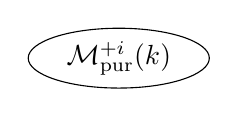
\begin{tikzpicture}[baseline=(m.base)]
\node (m) at (0,0) {$\mathcal{M}^{+i}_{\mathrm{pur}}(k)$};
\draw (0,0) ellipse (1.15 and .38);
\end{tikzpicture}}}
\]
où $M'_i$ est \deleted{\unsure{purement de poids}}\inserted{\uline{effectif}} pur de poids et niveau $i$.

\margin{\unsure{Exemp.} : si $i>n=\dim X$, alors $h^i(X)$ est \uline{de niveau} $\leq2n-i<i$.}

\deleted{\unsure{Ceci signifie}} Les motifs de \deleted{poids}\inserted{niveau} $\leq i$ sont ceux qui, modulo twist de Tate, ``proviennent'' des variétés $X\in V(k)$ de dimension $\leq i$. Ceci résulte du fait que $h(X)$ est de niveau $\leq\dim X$, et que \deleted{\unsure{d'ailleurs}} si $i\leq\dim X$, $h^i(X)\hookrightarrow h^i(Y)$, où $Y$ est une section linéaire de dim $i$ (au sens du ``th. de Lefschetz''). Autre interprétation en termes de cohomologie $\ell$-adique
\deleted{(en supposant $k$ alg. clos, ce qui est loisible, car la notion de niveau, \unsure{pureté de niveau}, est invariante par extension du corps de base)}
On regarde dans $H^i(\overline X,\mathbb{Q}_\ell)$ la ``filtration géométrique'' définie par
\[
\operatorname{Filt}^{j}H^i(X,\mathbb{Q}_\ell)
=\underset{U,\ U\text{ ouvert \unsure{tels que}}\ \operatorname{codim}(X-U)\geq j}{\unsure{\varinjlim|\lim}}
\operatorname{Ker}\bigl(H^i(X,\mathbb{Q}_\ell)\longrightarrow H^i(U,\mathbb{Q}_\ell)\bigr)
\]
\margin{\uline{Ex} Si $i\geq n=\dim X$\quad $h^i(X)$ est de niveau $\leq2n-i$.}
